\documentclass[onesided]{ccg-pset}

\course{MATH 6270}
\psnum{2}
\author{Colton Grainger}
\date{\today}


\begin{document}
\maketitle

\begin{note}[Conventions and Symbols]
    \label{conventions}
    \hfill
    \begin{itemize}
        \item We work with concrete categories $\cat{C}$, i.e., categories for which there exists a faithful functor $F \colon \cat{C} \inj \Set$ that is injective from the set% 
            \footnote{%
                At the risk of being evil, I'm requiring this collection of morphisms to be a set. This is about as much set theory as I'm prepared to handle. See also \url{https://en.wikipedia.org/wiki/Concrete_category}.
            }
            of morphisms $\cat{Mor(C)}$ in $\cat{C}$ to the set of functions $\cat{Map(Set)}$ in $\Set$).
    \end{itemize}
\end{note}

\begin{enumerate}
        \setcounter{enumi}{1}
    \item Given. Let $F(X)$, $F(Y)$ be free groups over the sets $X$, $Y$.

        To prove. If $F(X) \cong F(Y)$ are isomorphic as groups, then the sets $X \cong Y$ have the same cardinality.

\begin{proof}
    We will argue that the free group functor $F \colon \Set \to \Grp$ is a fully faithful functor, in order to see that the isomorphism $F(X) \xrightarrow{\cong} F(Y)$ is induced by a unique bijection $X \xrightarrow{\cong}Y$. See figure.

\end{proof}

    \begin{figure}[htpb]
        \centering
        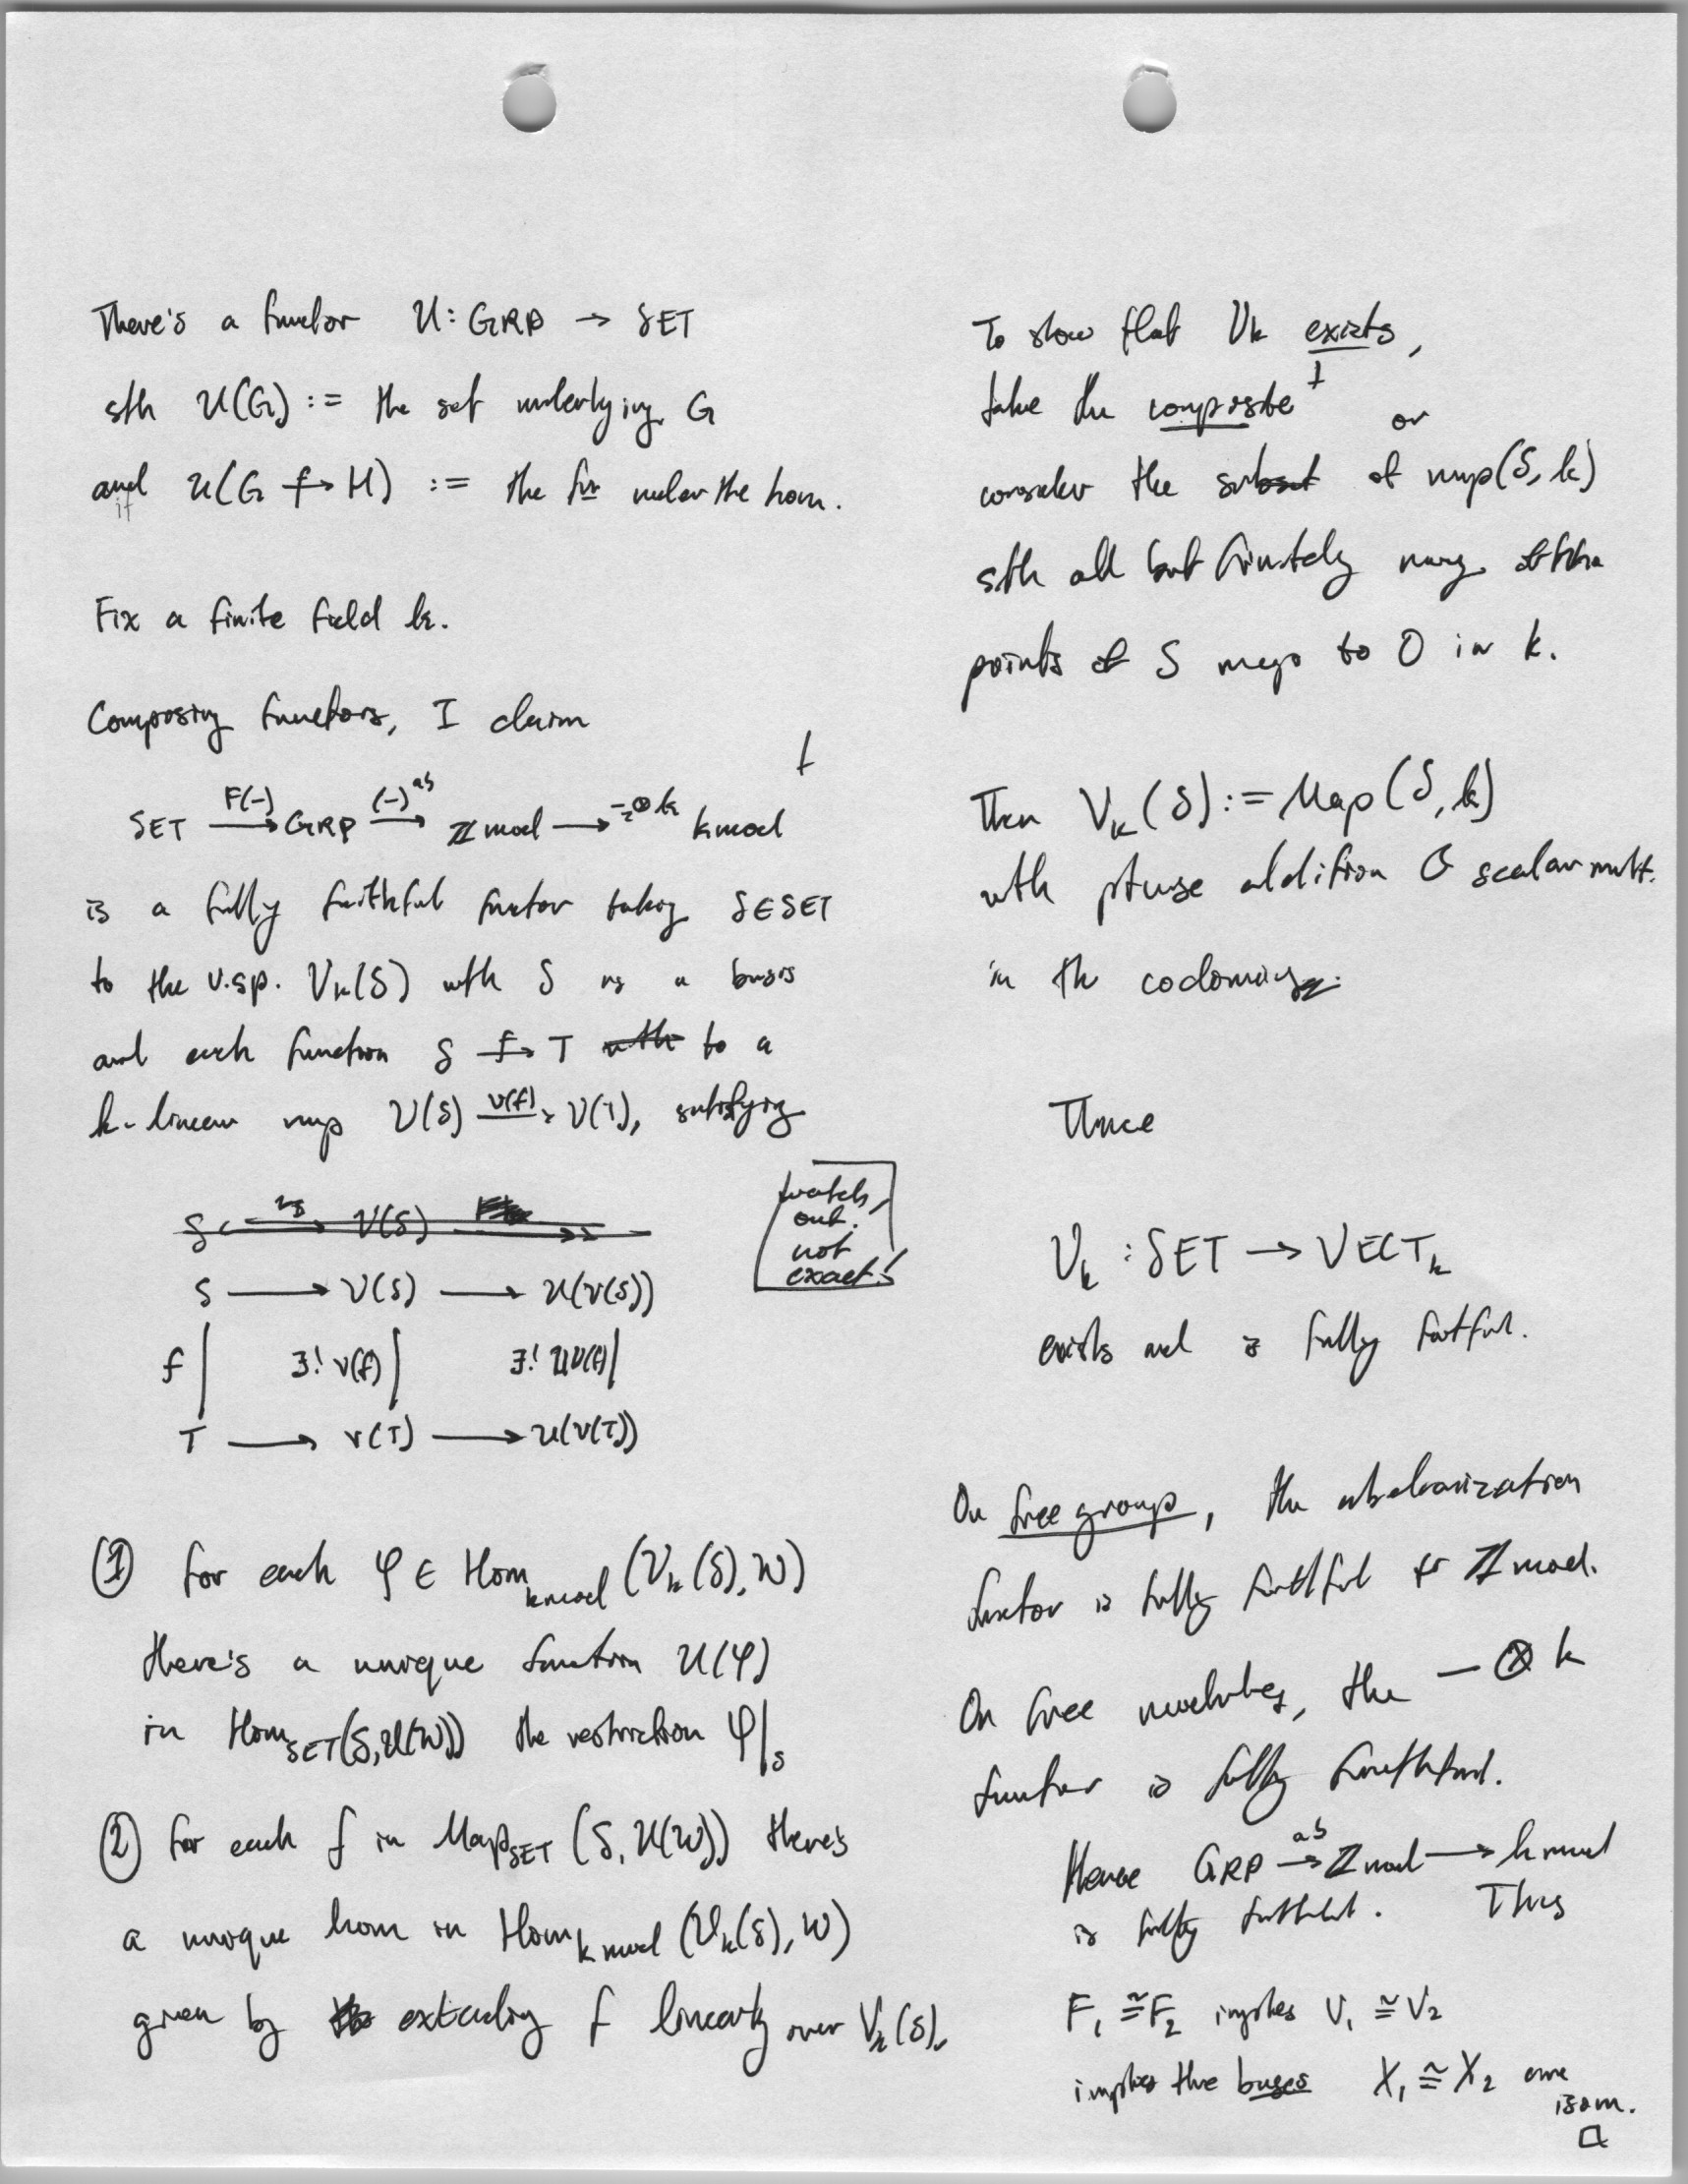
\includegraphics[width=0.8\linewidth]{20190911T0958.png}
        \caption{Sketch of proof}
        \label{}
    \end{figure}
\item Given. Consider a group presentation $G = \ang{X \mid R}$ with strictly more generators than relations: $\abs{X} > \abs{R}$.

    To prove. $G$ is infinite.

        \begin{proof}
            Define $Q = R \cup \set{\text{simple commutators }[x,y] \text{for all }x,y \in X}$. The normal closure of $Q$ includes the commutator subgroup of $\ang{X}$, which yields a quotient map $\ang{X \mid R} \surj \ang{X \mid Q}$ onto an abelian group. Let $Z$ denote the set of relations in $Q$ which are not simple commutators. From our hypothesis, $Z$ has cardinality strictly less than $X$. In the free abelian group $\Z\set{X}$, the relations in $Z$ produce a underdetermined system of $\Z$-linear relations on the generators in $X$. In the vector space $\Z\set{X} \otimes \Q$, the dimension of the subspace spanned by the solutions to these relations has strictly positive codimension. Thence the quotient of $\Z\set{X} \otimes \Q$ is infinite. Taking fibers over both projections yields the proposition.
        \end{proof}

    \item Given. Let $G = \ang{\set{a,b} : \set{a^n, b^m}}$ be a group presentation with the exponents $m,n \ge 2$.

        To prove. $G$ is infinite.
\begin{figure}[htpb]
    \centering
    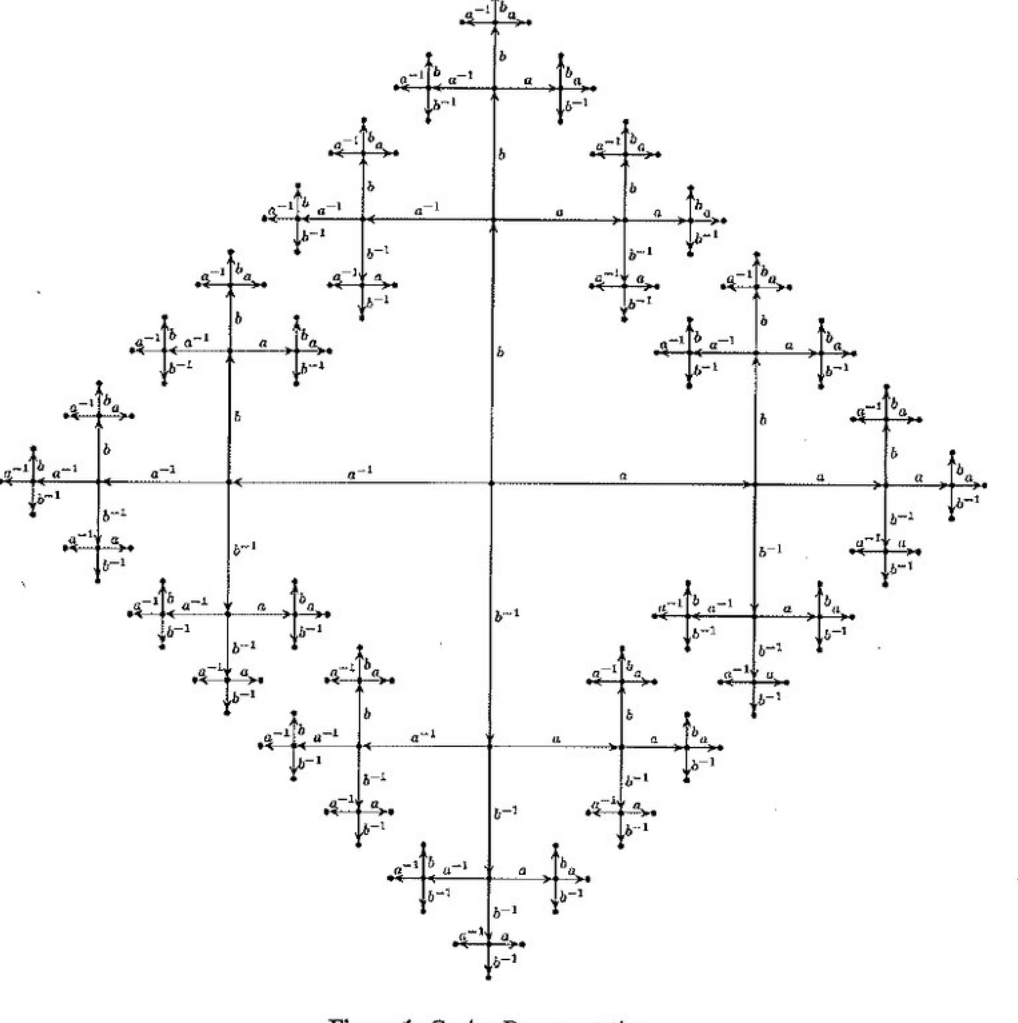
\includegraphics[width=0.25\linewidth]{2019-09-11-cayley.png}
    \caption{Cayley diagram for $F\paren{\set{a,b}}$}
    \label{fig:cayley}
\end{figure}
        \begin{proof}
            Consider the free group $F = F(\set{a,b})$ on two generators. Let $F$ act on itself by right translation. I claim the orbit of the normal subgroup $N = \ang{\set{w(a^n, b^m)^{g} : g \in F}}$ is infinite. 

            Recall two cosets $N\alpha$ and $N\beta$ coincide if and only if $\alpha\beta^{-1} \in N$. 

            Let $\alpha = [a,b]^{\nu}:=(aba^{-1}b^{-1})^{\nu}$ and $\beta = [a,b]^\mu$ for $\mu, \nu \in \Z$. Let $w \in N [a,b]^\mu$ be an arbitrary (non-empty) reduced word in the coset $N [a,b]^\mu$. We show that $\alpha\beta^{-1} \in N$ if and only if $\mu = \nu$. 

            Say $\mu \neq \nu$ and let $\bar{w}$ be a (nonempty) reduced word in $N$. Note $\alpha\beta^{-1}$ is not empty. Now, because $\bar{w}$ is a conjugate of some word $w(a^n, b^m)$ over the letters $a^n$ and $b^m$, either the first or last letter of $\bar{w}$ has exponent greater in magnitude than $1$, where $n, m >1$. However, both first and last letters of the reduced word $(aba^{-1}b^{-1})^{\nu}(aba^{-1}b^{-1})^{-\mu}$ has exponent no larger in magnitude than $1$. 

            We have shown the representative reduced words $\alpha\beta^{-1} \neq \bar{w}$ are not equal, hence $\alpha\beta^{-1}\not\in N$. If $\mu - \nu = 0$, we have the empty word $\alpha\beta^{-1} = \alpha\alpha^{-1} \in N$. 

            We have shown there are countably many cosets of $N$ in $F$. Hence the quotient $F/N$ is not finite.
        \end{proof}
\end{enumerate}

\end{document}
